\documentclass{mefsdp}
 
 
\setauthors{Jane Doe \and John Doe \and John Smith \and Jack Brown}
\setauthorsflat{Jane Doe, John Doe, John Smith, Jack Brown}
\settitle{title of the design project goes here in all capital letters and longer text may be subject to automatic line breaks}
\setcourseno{I}
\setyear{2020}
\setfaculty{Faculty of Engineering}
\setdepartment{Computer Engineering}
\setchair{Prof. Muhittin Gökmen}
\setdate{\today}
\setadvisor{Assoc. Prof. Şeniz Demir}

\newacronym{svm}{SVM}{Support Vector Machines}
\newacronym{ml}{ML}{Machine Learning}
\newacronym{dl}{DL}{Deep Learning}

\begin{document}
	
	\coverpage
	\descriptivetitle
	\acceptancepage
	\honestypledge

	
	\tableofcontents
	\listoffigures
	\listoftables
	\listofabbreviations
	
	\section{Introduction}
	
	First use: \gls{svm}. Second use: \gls{svm}.
	The introduction section should include general information about the project, the motivation of choosing this project, which will cover the broad impact of the project in terms of global, economic, environmental, societal, legal, health, and security context, and the global and environmental impact of the solution proposed. 
	
	\subsection{Motivation}
	
	In this part you should answer the following questions: “Why is it important to work on this project? How do people benefit from the outcomes of the  proposed project?
	
	\subsection{Broad impact}
	
	Explain the impact of the topic/solution method that you studied in terms of economic, societal, health, and security context. 
	
	\begin{table}[h]
		\centering
		\begin{tabular}{| c | c | c |}
			\hline
			\bfseries Year & \bfseries Method & \bfseries Dataset \\
			\hline
			1974 & Statistical Analysis & Human activity (100 persons) \\
			1986 & Structural Pattern Recognition & Text data (2000 words) \\
			1986 & Structural Pattern Recognition & Text data (2000 words) \\
			\hline
		\end{tabular}
	\caption[First sample table]{This is a sample table caption. Use Insert/Caption to add table captions. Table captions are provided at the top of the table.}
	\end{table}
	
	\subsubsection{Global Impact of the solution}
	What are the global and environmental impacts of the project? 
	
	\subsubsection{Economic Impact of the solution}
	What are the economic impacts of the project? 
	
	\subsubsection{Environmental Impact of the solution}
	What are the environmental impacts of the project?
	
	\subsubsection{Societal Impacts of the solution}
	What are the societal impacts of the project?
	
	\subsubsection{Legal Issues related to the project}
	What are the legal consequences and issues related with health, security, and business? Does it have any violation of human rights or intellectual property rights?s
	
	\section{Project Definition and Planning}
	Explain your project and provide details of your project planning in this section.
	\begin{figure}[h]
		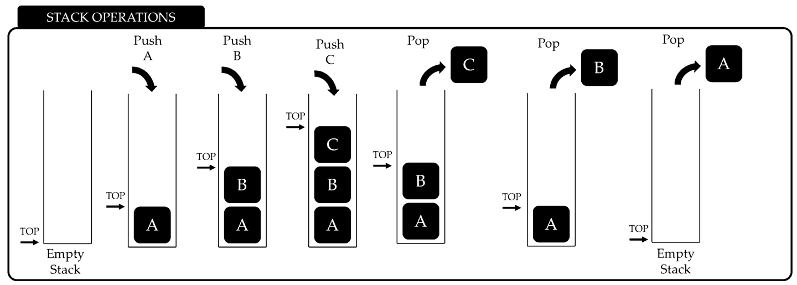
\includegraphics[scale=1]{../figures/sample_figure}
		\caption[First sample figure]{Sample figure. Use Insert/Caption to insert figure captions}
	\end{figure}

	In one dimension, the Gaussian function is the probability density function of the normal distribution. 
	
	\begin{equation}
		f(x) = \frac{1}{\sigma\sqrt{2\pi}}e^{\dfrac{-(x-\mu)^2}{2\sigma^2}}
	\end{equation}
	
	sometimes also called the frequency curve. The full width at half maximum for a Gaussian is found by finding the half-maximum points $x_0$.
	
	\subsection{Project Definition}
	Project definition. Describe your project in this section. Provide the project scope, functional and non-functional requirements of the project. 
	
	\subsection{Project Planning}
	Apply Work Breakdown Structure (WBS) to determine tasks and subtasks. Provide a GANTT chart with a time table, identify responsible person(s) for each task.   
	
	\begin{figure}[t]
		\centering
		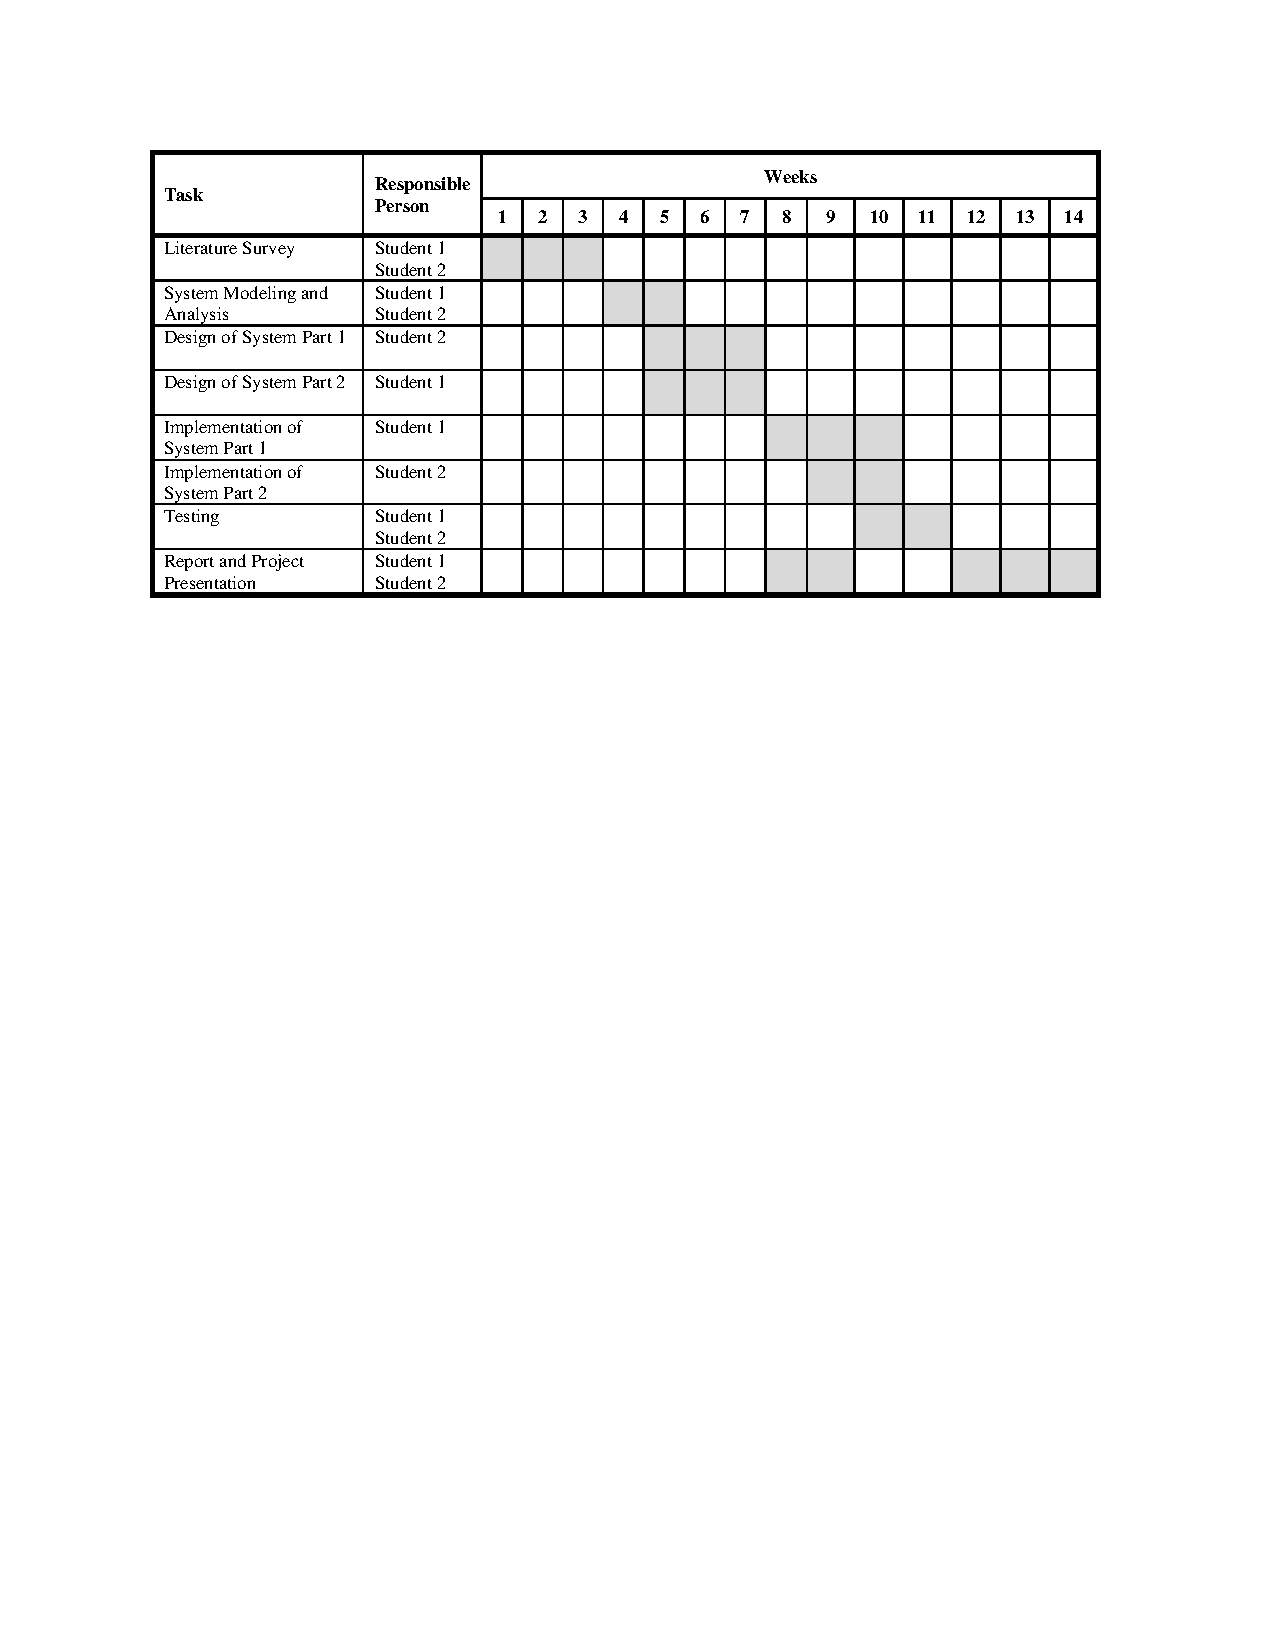
\includegraphics[scale=.85]{../figures/gantt}
		\caption{Sample project plan for 14 weeks}
	\end{figure}
	\newpage
	\subsubsection{Aim of the project}
	Describe the aim of the project in one paragraph.
	
	\subsubsection{Project definition}
	Describe the content of the project. 
	
	\subsubsection{Use Cases}
	Provide UML use case diagrams by specifying systems, actors, use cases and relationships. \cite{kahneman2011thinking}
	
	\subsubsection{Success Criteria}
	Describe the success criteria of the project. 
	
	\subsubsection{Project time and resource estimation}
	Provide time (Month) and effort (Person/Month) estimation of the project. Describe how you estimated them. Provide a cost estimate of the project by considering the human resources, hardware and software resources etc.
	
	\subsubsection{Solution Strategies and Applicable Methods}
	Describe the alternative approaches to solve the problem. After comparing their advantageous and disadvantageous, explain the method you decided to use to solve each sub problem in the project, together with why you selected this method. \gls{dl} and \gls{dl}
	
	\subsubsection{Risk Analysis}
	Describe what are the risks of completing the project successfully. Identify the risks, their impacts and likelihoods. Describe how to avoid these risks and what to do if the risk occurs. \cite{duan2017question}
	
	\subsubsection{Tools Needed}
	Describe which software and hardware tools you need in the project.
	\cite{rothstein2017color}
	
	
	\section{Theoretical Background}
	You will define your problem in this section and add subheadings as needed. If you give your problem description and solution methodology in this section, you may need to change the title of this section. We usually write a couple of sentence in this part that explains what we will discuss in this section. For example: We will first provide the problem definition of our study (write you topic here), and then give the mathematical model that we propose as a solution method in this section.
	
	\subsection{Literature Survey}
	Provide a survey of the relevant literature. A bibliography (or references) is a selected list of all books, articles, and other source material related to the project and is always in alphabetical order, with the author's last name first. You have to cite a reference within the document as the authors last name (year). For example, “Jones (1969) show that ....”. If the article has only one author, then the citation will be Jones (1969); if the article has two authors, then the citation will be Jones and Brown (1969); for all others, the citation will be Jones et al. (1969). For example; the first reference of this document is cited as Bass (1969), the second one is cited as Bass and Bass (2004), and the third one is cited as DeKimpe et al. (2000). If the citation is in parentheses, then the citations will be (Bass, 1969), (Jones and Brown, 1969) and (Bass et al., 1969) for the above example, respectively. 
	\cite{DBLP:journals/corr/VaswaniSPUJGKP17}
	
	\subsection{Solution Method (Change this title according to your solution method)}
	Provide detailed solution method here.
	
	
	\section{Analysis and Modeling}
	We first give details about the project that we selected. We define the scope of the project, functional and non-functional requirements. Then, we give details of the problem that the company was experiencing. Finally, we provide detailed analysis that we conducted by using real-life data obtained from the company. 
	
	\subsection{System Factors}
	Explain factors that can affect the system.
	
	\subsection{How System Works}
	Explain how your system will work
	
	\subsubsection{Modelling}
	Explanation of system model.
	
	\subsubsection{System Architecture }
	Explanation of system architecture.
	
	\subsubsection{UML (Unified Modeling Language) Diagrams}
	
	\section{Design, implementation and testing}
	Explain design, implementation and testing of your system in detail.
	
	\subsection{Design}
	Explanation of the design of your system.
	
	\subsection{Implementation}
	Explanation of the implementation of your system.
	
	\subsection{Testing}
	Explanation of the testing of your system.
	
	\section{Results}
	Explain your results.
	
	\section{Conclusion}
	Briefly explain the problem you studied, the solution method you proposed and your experience in the implementation. Then, please proceed to subsections and explain the requirements in details. 
	
	\subsection{Life-Long Learning}
	Identify additional knowledge, skills, and attitudes that you needed to complete the project. In the context of the project, which tools and methods did you learn by yourself?  From which sources did you learn them? How difficult was for you to learn these topics by yourself? How did you manage to collect the relevant information? Answer all the questions.
	
	\subsection{Professional and ethical responsibilities of engineers}
	Define professional and ethical responsibilities you followed during your design process. What are the professional and ethical standards you used in the project? Is there an ethics code or code of conduct? Answer all the questions.
	
	\subsection{Contemporary Issues}
	Evaluate you project experience in terms of contemporary issues related to the problem that you studied. What kind of contemporary tools you have used throughout your project? Analyze the contemporary issues related to the future of the field that you work in this project. What will change in the products, services, or processes in the next ten, twenty, or fifty years, with emerging technologies such as 3D printers, big data analytics, nanotechnology, internet of things, quantum computing, biotechnology, artificial intelligence, cognitive science, and robotics?
	
	\subsection{Team Work}
	During your design project experience, describe the team work that you have participated. Give positions and majors of the people in the company that you worked with. Evaluate the composition, organization, and performance of your team. Describe how you shared the load in terms of the project tasks. 
	
	
	
	\bibliographystyle{apalike}
	\bibliography{../bibliography/references}
\end{document}